
%(BEGIN_QUESTION)
% Copyright 2011, Tony R. Kuphaldt, released under the Creative Commons Attribution License (v 1.0)
% This means you may do almost anything with this work of mine, so long as you give me proper credit

%A {\it Programmable Logic Controller} or {\it PLC} is an industrial control computer designed to input and output many types of signals.  To handle different signal types (on/off, analog, digital networking), large-scale PLCs use different ``cards'' that plug into a common frame to provide I/O capacity to the processor:

En PLS er en styringsenhet som skal behandler mange typer in- og utgangssignaler. For å få dette til er det vanlig å bruke ulike løsninger for tilkobling av ekstrakort. 

$$\includegraphics[width=15.5cm]{i02271x01.eps}$$

%Read selected portions of the Allen-Bradley PLC ``1756 ControlLogix I/O Modules'' publication (document 1756-TD002A-EN-E, May 2009), and answer the following questions:

Les i instruskjonsmanualen for V200-18-E2B, og svar på følgende spørsmål. 

\vskip 10pt

%Locate the sample 4-20 mA device wiring diagrams for the 1756-IF6CIS ``sourcing current loop analog input module'', identifying the different types of 4-20 mA field devices supported.
Finn ut hvordan h.h.v 0-10 V og 4-20mA transmittere tilkobles kortet. 

\vskip 10pt

Finn ut hvilke inngangsområder som kan brukes av kortet, og hvor mange steg de deles opp i. 

\vskip 10pt

%Calculate the number of counts per milliamp of signal with this analog input card, and also the resolution (mA per count).
Regn ut antal steg per milliamper av signal på dette kortet. Finn også oppløsningen i mA pr. steg

\vskip 10pt

%Calculate the ``User counts'' value for a 8.51 mA signal value input to this analog card.
Regn ut antal steg for et signal på 8.51 mA tilført inngangen. 


\vskip 10pt

%Calculate the mA current signal value at a ``User counts'' value of +4592.

Regn ut hvor stort inngangsignal i mA når antal steg på inngangen er +754

\underbar{file i02271}
%(END_QUESTION)




%(BEGIN_ANSWER)

%Pages 28 and 29: this card may connect to loop-powered (2-wire) 4-20 mA devices as well as self-powered (4-wire) devices.  Three connection terminals are provided per channel: a positive voltage terminal (VOUT), an input terminal (IN), and a ground (RTN).

\vskip 10pt

%3106.8 counts per mA (equivalent to 0.3 microamps per count).

%(END_ANSWER)





%(BEGIN_NOTES)

%Pages 28 and 29: this card may connect to loop-powered (2-wire) 4-20 mA devices as well as self-powered (4-wire) devices.  Three connection terminals are provided per channel: a positive voltage terminal (VOUT), an input terminal (IN), and a ground (RTN).

\vskip 10pt

%Page 29: 0 to 21.09376 mA ; -32768 to +32767 counts.  This is clearly a 16-bit ADC expressing its count value as a signed integer (2's complement notation).

\vskip 10pt

${65535 \over 21.09376}= 3106.84$ counts per mA (equivalent to 0.3 microamps per count).

\vskip 10pt

8.51 mA = ${8.51 \over 21.09376}$ = 40.343\% of 65535 count span = 26439 counts above bottom = -6329 counts (-6328.766312 calculated)

\vskip 10pt

4592 counts = ${4592 - (-32768) \over 65535}$ = 57.0077\% of 21.09376 mA span = 12.02506864 mA

%INDEX% PLC, I/O: analog resolution and scaling
%INDEX% Reading assignment: Allen-Bradley 1756 ControlLogix I/O Modules publication

%(END_NOTES)

